\PassOptionsToPackage{dvipsnames,table}{xcolor}
\documentclass[10pt]{beamer}
\usepackage{Cours}

\begin{document}


\newcounter{numchap}
\setcounter{numchap}{1}
\newcounter{numframe}
\setcounter{numframe}{0}
\newcommand{\mframe}[1]{\frametitle{#1} \addtocounter{numframe}{1}}
\newcommand{\cnum}{\fbox{\textcolor{yellow}{\textbf{C\thenumchap}}}~}
\newcommand{\makess}[1]{\section{#1} \label{ss\thesection}}
\newcommand{\stitle}{\textcolor{yellow}{\textbf{\thesection. \nameref{ss\thesection}}}}

\definecolor{codebg}{gray}{0.90}
\definecolor{grispale}{gray}{0.95}
\definecolor{fluo}{rgb}{1,0.96,0.62}
\newminted[langageC]{c}{linenos=true,escapeinside=||,highlightcolor=fluo,tabsize=2,breaklines=true}
\newminted[codepython]{python}{linenos=true,escapeinside=||,highlightcolor=fluo,tabsize=2,breaklines=true}
% Inclusion complète (ou partiel en indiquant premiere et dernière ligne) d'un fichier C
\newcommand{\inputC}[3]{\begin{mdframed}[backgroundcolor=codebg] \inputminted[breaklines=true,fontsize=#3,linenos=true,highlightcolor=fluo,tabsize=2,highlightlines={#2}]{c}{#1} \end{mdframed}}
\newcommand{\inputpartC}[5]{\begin{mdframed}[backgroundcolor=codebg] \inputminted[breaklines=true,fontsize=#3,linenos=true,highlightcolor=fluo,tabsize=2,highlightlines={#2},firstline=#4,lastline=#5,firstnumber=1]{c}{#1} \end{mdframed}}
\newcommand{\inputpython}[3]{\begin{mdframed}[backgroundcolor=codebg] \inputminted[breaklines=true,fontsize=#3,linenos=true,highlightcolor=fluo,tabsize=2,highlightlines={#2}]{python}{#1} \end{mdframed}}
\newcommand{\inputpartOCaml}[5]{\begin{mdframed}[backgroundcolor=codebg] \inputminted[breaklines=true,fontsize=#3,linenos=true,highlightcolor=fluo,tabsize=2,highlightlines={#2},firstline=#4,lastline=#5,firstnumber=1]{OCaml}{#1} \end{mdframed}}
\BeforeBeginEnvironment{minted}{\begin{mdframed}[backgroundcolor=codebg]}
\AfterEndEnvironment{minted}{\end{mdframed}}
\newcommand{\kw}[1]{\textcolor{blue}{\tt #1}}

\newtcolorbox{rcadre}[4]{halign=center,colback={#1},colframe={#2},width={#3cm},height={#4cm},valign=center,boxrule=1pt,left=0pt,right=0pt}
\newtcolorbox{cadre}[4]{halign=center,colback={#1},colframe={#2},arc=0mm,width={#3cm},height={#4cm},valign=center,boxrule=1pt,left=0pt,right=0pt}
\newcommand{\myem}[1]{\colorbox{fluo}{#1}}
\mdfsetup{skipabove=1pt,skipbelow=-2pt}



% Noeud dans un cadre pour les arbres
\newcommand{\noeud}[2]{\Tr{\fbox{\textcolor{#1}{\tt #2}}}}

\newcommand{\htmlmode}{\lstset{language=html,numbers=left, tabsize=4, frame=single, breaklines=true, keywordstyle=\ttfamily, basicstyle=\small,
   numberstyle=\tiny\ttfamily, framexleftmargin=0mm, backgroundcolor=\color{grispale}, xleftmargin=12mm,showstringspaces=false}}
\newcommand{\pythonmode}{\lstset{
   language=python,
   linewidth=\linewidth,
   numbers=left,
   tabsize=4,
   frame=single,
   breaklines=true,
   keywordstyle=\ttfamily\color{blue},
   basicstyle=\small,
   numberstyle=\tiny\ttfamily,
   framexleftmargin=-2mm,
   numbersep=-0.5mm,
   backgroundcolor=\color{codebg},
   xleftmargin=-1mm, 
   showstringspaces=false,
   commentstyle=\color{gray},
   stringstyle=\color{OliveGreen},
   emph={turtle,Screen,Turtle},
   emphstyle=\color{RawSienna},
   morekeywords={setheading,goto,backward,forward,left,right,pendown,penup,pensize,color,speed,hideturtle,showturtle,forward}}
   }
   \newcommand{\Cmode}{\lstset{
      language=[ANSI]C,
      linewidth=\linewidth,
      numbers=left,
      tabsize=4,
      frame=single,
      breaklines=true,
      keywordstyle=\ttfamily\color{blue},
      basicstyle=\small,
      numberstyle=\tiny\ttfamily,
      framexleftmargin=0mm,
      numbersep=2mm,
      backgroundcolor=\color{codebg},
      xleftmargin=0mm, 
      showstringspaces=false,
      commentstyle=\color{gray},
      stringstyle=\color{OliveGreen},
      emphstyle=\color{RawSienna},
      escapechar=\|,
      morekeywords={}}
      }
\newcommand{\bashmode}{\lstset{language=bash,numbers=left, tabsize=2, frame=single, breaklines=true, basicstyle=\ttfamily,
   numberstyle=\tiny\ttfamily, framexleftmargin=0mm, backgroundcolor=\color{grispale}, xleftmargin=12mm, showstringspaces=false}}
\newcommand{\exomode}{\lstset{language=python,numbers=left, tabsize=2, frame=single, breaklines=true, basicstyle=\ttfamily,
   numberstyle=\tiny\ttfamily, framexleftmargin=13mm, xleftmargin=12mm, basicstyle=\small, showstringspaces=false}}
   
   
  
%tei pour placer les images
%tei{nom de l’image}{échelle de l’image}{sens}{texte a positionner}
%sens ="1" (droite) ou "2" (gauche)
\newlength{\ltxt}
\newcommand{\tei}[4]{
\setlength{\ltxt}{\linewidth}
\setbox0=\hbox{\includegraphics[scale=#2]{#1}}
\addtolength{\ltxt}{-\wd0}
\addtolength{\ltxt}{-10pt}
\ifthenelse{\equal{#3}{1}}{
\begin{minipage}{\wd0}
\includegraphics[scale=#2]{#1}
\end{minipage}
\hfill
\begin{minipage}{\ltxt}
#4
\end{minipage}
}{
\begin{minipage}{\ltxt}
#4
\end{minipage}
\hfill
\begin{minipage}{\wd0}
\includegraphics[scale=#2]{#1}
\end{minipage}
}
}

%Juxtaposition d'une image pspciture et de texte 
%#1: = code pstricks de l'image
%#2: largeur de l'image
%#3: hauteur de l'image
%#4: Texte à écrire
\newcommand{\ptp}[4]{
\setlength{\ltxt}{\linewidth}
\addtolength{\ltxt}{-#2 cm}
\addtolength{\ltxt}{-0.1 cm}
\begin{minipage}[b][#3 cm][t]{\ltxt}
#4
\end{minipage}\hfill
\begin{minipage}[b][#3 cm][c]{#2 cm}
#1
\end{minipage}\par
}



%Macros pour les graphiques
\psset{linewidth=0.5\pslinewidth,PointSymbol=x}
\setlength{\fboxrule}{0.5pt}
\newcounter{tempangle}

%Marque la longueur du segment d'extrémité  #1 et  #2 avec la valeur #3, #4 est la distance par rapport au segment (en %age de la valeur de celui ci) et #5 l'orientation du marquage : +90 ou -90
\newcommand{\afflong}[5]{
\pstRotation[RotAngle=#4,PointSymbol=none,PointName=none]{#1}{#2}[X] 
\pstHomO[PointSymbol=none,PointName=none,HomCoef=#5]{#1}{X}[Y]
\pstTranslation[PointSymbol=none,PointName=none]{#1}{#2}{Y}[Z]
 \ncline{|<->|,linewidth=0.25\pslinewidth}{Y}{Z} \ncput*[nrot=:U]{\footnotesize{#3}}
}
\newcommand{\afflongb}[3]{
\ncline{|<->|,linewidth=0}{#1}{#2} \naput*[nrot=:U]{\footnotesize{#3}}
}

%Construis le point #4 situé à #2 cm du point #1 avant un angle #3 par rapport à l'horizontale. #5 = liste de paramètre
\newcommand{\lsegment}[5]{\pstGeonode[PointSymbol=none,PointName=none](0,0){O'}(#2,0){I'} \pstTranslation[PointSymbol=none,PointName=none]{O'}{I'}{#1}[J'] \pstRotation[RotAngle=#3,PointSymbol=x,#5]{#1}{J'}[#4]}
\newcommand{\tsegment}[5]{\pstGeonode[PointSymbol=none,PointName=none](0,0){O'}(#2,0){I'} \pstTranslation[PointSymbol=none,PointName=none]{O'}{I'}{#1}[J'] \pstRotation[RotAngle=#3,PointSymbol=x,#5]{#1}{J'}[#4] \pstLineAB{#4}{#1}}

%Construis le point #4 situé à #3 cm du point #1 et faisant un angle de  90° avec la droite (#1,#2) #5 = liste de paramètre
\newcommand{\psegment}[5]{
\pstGeonode[PointSymbol=none,PointName=none](0,0){O'}(#3,0){I'}
 \pstTranslation[PointSymbol=none,PointName=none]{O'}{I'}{#1}[J']
 \pstInterLC[PointSymbol=none,PointName=none]{#1}{#2}{#1}{J'}{M1}{M2} \pstRotation[RotAngle=-90,PointSymbol=x,#5]{#1}{M1}[#4]
  }
  
%Construis le point #4 situé à #3 cm du point #1 et faisant un angle de  #5° avec la droite (#1,#2) #6 = liste de paramètre
\newcommand{\mlogo}[6]{
\pstGeonode[PointSymbol=none,PointName=none](0,0){O'}(#3,0){I'}
 \pstTranslation[PointSymbol=none,PointName=none]{O'}{I'}{#1}[J']
 \pstInterLC[PointSymbol=none,PointName=none]{#1}{#2}{#1}{J'}{M1}{M2} \pstRotation[RotAngle=#5,PointSymbol=x,#6]{#1}{M2}[#4]
  }

% Construis un triangle avec #1=liste des 3 sommets séparés par des virgules, #2=liste des 3 longueurs séparés par des virgules, #3 et #4 : paramètre d'affichage des 2e et 3 points et #5 : inclinaison par rapport à l'horizontale
%autre macro identique mais sans tracer les segments joignant les sommets
\noexpandarg
\newcommand{\Triangleccc}[5]{
\StrBefore{#1}{,}[\pointA]
\StrBetween[1,2]{#1}{,}{,}[\pointB]
\StrBehind[2]{#1}{,}[\pointC]
\StrBefore{#2}{,}[\coteA]
\StrBetween[1,2]{#2}{,}{,}[\coteB]
\StrBehind[2]{#2}{,}[\coteC]
\tsegment{\pointA}{\coteA}{#5}{\pointB}{#3} 
\lsegment{\pointA}{\coteB}{0}{Z1}{PointSymbol=none, PointName=none}
\lsegment{\pointB}{\coteC}{0}{Z2}{PointSymbol=none, PointName=none}
\pstInterCC{\pointA}{Z1}{\pointB}{Z2}{\pointC}{Z3} 
\pstLineAB{\pointA}{\pointC} \pstLineAB{\pointB}{\pointC}
\pstSymO[PointName=\pointC,#4]{C}{C}[C]
}
\noexpandarg
\newcommand{\TrianglecccP}[5]{
\StrBefore{#1}{,}[\pointA]
\StrBetween[1,2]{#1}{,}{,}[\pointB]
\StrBehind[2]{#1}{,}[\pointC]
\StrBefore{#2}{,}[\coteA]
\StrBetween[1,2]{#2}{,}{,}[\coteB]
\StrBehind[2]{#2}{,}[\coteC]
\tsegment{\pointA}{\coteA}{#5}{\pointB}{#3} 
\lsegment{\pointA}{\coteB}{0}{Z1}{PointSymbol=none, PointName=none}
\lsegment{\pointB}{\coteC}{0}{Z2}{PointSymbol=none, PointName=none}
\pstInterCC[PointNameB=none,PointSymbolB=none,#4]{\pointA}{Z1}{\pointB}{Z2}{\pointC}{Z1} 
}


% Construis un triangle avec #1=liste des 3 sommets séparés par des virgules, #2=liste formée de 2 longueurs et d'un angle séparés par des virgules, #3 et #4 : paramètre d'affichage des 2e et 3 points et #5 : inclinaison par rapport à l'horizontale
%autre macro identique mais sans tracer les segments joignant les sommets
\newcommand{\Trianglecca}[5]{
\StrBefore{#1}{,}[\pointA]
\StrBetween[1,2]{#1}{,}{,}[\pointB]
\StrBehind[2]{#1}{,}[\pointC]
\StrBefore{#2}{,}[\coteA]
\StrBetween[1,2]{#2}{,}{,}[\coteB]
\StrBehind[2]{#2}{,}[\angleA]
\tsegment{\pointA}{\coteA}{#5}{\pointB}{#3} 
\setcounter{tempangle}{#5}
\addtocounter{tempangle}{\angleA}
\tsegment{\pointA}{\coteB}{\thetempangle}{\pointC}{#4}
\pstLineAB{\pointB}{\pointC}
}
\newcommand{\TriangleccaP}[5]{
\StrBefore{#1}{,}[\pointA]
\StrBetween[1,2]{#1}{,}{,}[\pointB]
\StrBehind[2]{#1}{,}[\pointC]
\StrBefore{#2}{,}[\coteA]
\StrBetween[1,2]{#2}{,}{,}[\coteB]
\StrBehind[2]{#2}{,}[\angleA]
\lsegment{\pointA}{\coteA}{#5}{\pointB}{#3} 
\setcounter{tempangle}{#5}
\addtocounter{tempangle}{\angleA}
\lsegment{\pointA}{\coteB}{\thetempangle}{\pointC}{#4}
}

% Construis un triangle avec #1=liste des 3 sommets séparés par des virgules, #2=liste formée de 1 longueurs et de deux angle séparés par des virgules, #3 et #4 : paramètre d'affichage des 2e et 3 points et #5 : inclinaison par rapport à l'horizontale
%autre macro identique mais sans tracer les segments joignant les sommets
\newcommand{\Trianglecaa}[5]{
\StrBefore{#1}{,}[\pointA]
\StrBetween[1,2]{#1}{,}{,}[\pointB]
\StrBehind[2]{#1}{,}[\pointC]
\StrBefore{#2}{,}[\coteA]
\StrBetween[1,2]{#2}{,}{,}[\angleA]
\StrBehind[2]{#2}{,}[\angleB]
\tsegment{\pointA}{\coteA}{#5}{\pointB}{#3} 
\setcounter{tempangle}{#5}
\addtocounter{tempangle}{\angleA}
\lsegment{\pointA}{1}{\thetempangle}{Z1}{PointSymbol=none, PointName=none}
\setcounter{tempangle}{#5}
\addtocounter{tempangle}{180}
\addtocounter{tempangle}{-\angleB}
\lsegment{\pointB}{1}{\thetempangle}{Z2}{PointSymbol=none, PointName=none}
\pstInterLL[#4]{\pointA}{Z1}{\pointB}{Z2}{\pointC}
\pstLineAB{\pointA}{\pointC}
\pstLineAB{\pointB}{\pointC}
}
\newcommand{\TrianglecaaP}[5]{
\StrBefore{#1}{,}[\pointA]
\StrBetween[1,2]{#1}{,}{,}[\pointB]
\StrBehind[2]{#1}{,}[\pointC]
\StrBefore{#2}{,}[\coteA]
\StrBetween[1,2]{#2}{,}{,}[\angleA]
\StrBehind[2]{#2}{,}[\angleB]
\lsegment{\pointA}{\coteA}{#5}{\pointB}{#3} 
\setcounter{tempangle}{#5}
\addtocounter{tempangle}{\angleA}
\lsegment{\pointA}{1}{\thetempangle}{Z1}{PointSymbol=none, PointName=none}
\setcounter{tempangle}{#5}
\addtocounter{tempangle}{180}
\addtocounter{tempangle}{-\angleB}
\lsegment{\pointB}{1}{\thetempangle}{Z2}{PointSymbol=none, PointName=none}
\pstInterLL[#4]{\pointA}{Z1}{\pointB}{Z2}{\pointC}
}

%Construction d'un cercle de centre #1 et de rayon #2 (en cm)
\newcommand{\Cercle}[2]{
\lsegment{#1}{#2}{0}{Z1}{PointSymbol=none, PointName=none}
\pstCircleOA{#1}{Z1}
}

%construction d'un parallélogramme #1 = liste des sommets, #2 = liste contenant les longueurs de 2 côtés consécutifs et leurs angles;  #3, #4 et #5 : paramètre d'affichage des sommets #6 inclinaison par rapport à l'horizontale 
% meme macro sans le tracé des segements
\newcommand{\Para}[6]{
\StrBefore{#1}{,}[\pointA]
\StrBetween[1,2]{#1}{,}{,}[\pointB]
\StrBetween[2,3]{#1}{,}{,}[\pointC]
\StrBehind[3]{#1}{,}[\pointD]
\StrBefore{#2}{,}[\longueur]
\StrBetween[1,2]{#2}{,}{,}[\largeur]
\StrBehind[2]{#2}{,}[\angle]
\tsegment{\pointA}{\longueur}{#6}{\pointB}{#3} 
\setcounter{tempangle}{#6}
\addtocounter{tempangle}{\angle}
\tsegment{\pointA}{\largeur}{\thetempangle}{\pointD}{#5}
\pstMiddleAB[PointName=none,PointSymbol=none]{\pointB}{\pointD}{Z1}
\pstSymO[#4]{Z1}{\pointA}[\pointC]
\pstLineAB{\pointB}{\pointC}
\pstLineAB{\pointC}{\pointD}
}
\newcommand{\ParaP}[6]{
\StrBefore{#1}{,}[\pointA]
\StrBetween[1,2]{#1}{,}{,}[\pointB]
\StrBetween[2,3]{#1}{,}{,}[\pointC]
\StrBehind[3]{#1}{,}[\pointD]
\StrBefore{#2}{,}[\longueur]
\StrBetween[1,2]{#2}{,}{,}[\largeur]
\StrBehind[2]{#2}{,}[\angle]
\lsegment{\pointA}{\longueur}{#6}{\pointB}{#3} 
\setcounter{tempangle}{#6}
\addtocounter{tempangle}{\angle}
\lsegment{\pointA}{\largeur}{\thetempangle}{\pointD}{#5}
\pstMiddleAB[PointName=none,PointSymbol=none]{\pointB}{\pointD}{Z1}
\pstSymO[#4]{Z1}{\pointA}[\pointC]
}


%construction d'un cerf-volant #1 = liste des sommets, #2 = liste contenant les longueurs de 2 côtés consécutifs et leurs angles;  #3, #4 et #5 : paramètre d'affichage des sommets #6 inclinaison par rapport à l'horizontale 
% meme macro sans le tracé des segements
\newcommand{\CerfVolant}[6]{
\StrBefore{#1}{,}[\pointA]
\StrBetween[1,2]{#1}{,}{,}[\pointB]
\StrBetween[2,3]{#1}{,}{,}[\pointC]
\StrBehind[3]{#1}{,}[\pointD]
\StrBefore{#2}{,}[\longueur]
\StrBetween[1,2]{#2}{,}{,}[\largeur]
\StrBehind[2]{#2}{,}[\angle]
\tsegment{\pointA}{\longueur}{#6}{\pointB}{#3} 
\setcounter{tempangle}{#6}
\addtocounter{tempangle}{\angle}
\tsegment{\pointA}{\largeur}{\thetempangle}{\pointD}{#5}
\pstOrtSym[#4]{\pointB}{\pointD}{\pointA}[\pointC]
\pstLineAB{\pointB}{\pointC}
\pstLineAB{\pointC}{\pointD}
}

%construction d'un quadrilatère quelconque #1 = liste des sommets, #2 = liste contenant les longueurs des 4 côtés et l'angle entre 2 cotés consécutifs  #3, #4 et #5 : paramètre d'affichage des sommets #6 inclinaison par rapport à l'horizontale 
% meme macro sans le tracé des segements
\newcommand{\Quadri}[6]{
\StrBefore{#1}{,}[\pointA]
\StrBetween[1,2]{#1}{,}{,}[\pointB]
\StrBetween[2,3]{#1}{,}{,}[\pointC]
\StrBehind[3]{#1}{,}[\pointD]
\StrBefore{#2}{,}[\coteA]
\StrBetween[1,2]{#2}{,}{,}[\coteB]
\StrBetween[2,3]{#2}{,}{,}[\coteC]
\StrBetween[3,4]{#2}{,}{,}[\coteD]
\StrBehind[4]{#2}{,}[\angle]
\tsegment{\pointA}{\coteA}{#6}{\pointB}{#3} 
\setcounter{tempangle}{#6}
\addtocounter{tempangle}{\angle}
\tsegment{\pointA}{\coteD}{\thetempangle}{\pointD}{#5}
\lsegment{\pointB}{\coteB}{0}{Z1}{PointSymbol=none, PointName=none}
\lsegment{\pointD}{\coteC}{0}{Z2}{PointSymbol=none, PointName=none}
\pstInterCC[PointNameA=none,PointSymbolA=none,#4]{\pointB}{Z1}{\pointD}{Z2}{Z3}{\pointC} 
\pstLineAB{\pointB}{\pointC}
\pstLineAB{\pointC}{\pointD}
}


% Définition des colonnes centrées ou à droite pour tabularx
\newcolumntype{Y}{>{\centering\arraybackslash}X}
\newcolumntype{Z}{>{\flushright\arraybackslash}X}

%Les pointillés à remplir par les élèves
\newcommand{\po}[1]{\makebox[#1 cm]{\dotfill}}
\newcommand{\lpo}[1][3]{%
\multido{}{#1}{\makebox[\linewidth]{\dotfill}
}}

%Liste des pictogrammes utilisés sur la fiche d'exercice ou d'activités
\newcommand{\bombe}{\faBomb}
\newcommand{\livre}{\faBook}
\newcommand{\calculatrice}{\faCalculator}
\newcommand{\oral}{\faCommentO}
\newcommand{\surfeuille}{\faEdit}
\newcommand{\ordinateur}{\faLaptop}
\newcommand{\ordi}{\faDesktop}
\newcommand{\ciseaux}{\faScissors}
\newcommand{\danger}{\faExclamationTriangle}
\newcommand{\out}{\faSignOut}
\newcommand{\cadeau}{\faGift}
\newcommand{\flash}{\faBolt}
\newcommand{\lumiere}{\faLightbulb}
\newcommand{\compas}{\dsmathematical}
\newcommand{\calcullitteral}{\faTimesCircleO}
\newcommand{\raisonnement}{\faCogs}
\newcommand{\recherche}{\faSearch}
\newcommand{\rappel}{\faHistory}
\newcommand{\video}{\faFilm}
\newcommand{\capacite}{\faPuzzlePiece}
\newcommand{\aide}{\faLifeRing}
\newcommand{\loin}{\faExternalLink}
\newcommand{\groupe}{\faUsers}
\newcommand{\bac}{\faGraduationCap}
\newcommand{\histoire}{\faUniversity}
\newcommand{\coeur}{\faSave}
\newcommand{\python}{\faPython}
\newcommand{\os}{\faMicrochip}
\newcommand{\rd}{\faCubes}
\newcommand{\data}{\faColumns}
\newcommand{\web}{\faCode}
\newcommand{\prog}{\faFile}
\newcommand{\algo}{\faCogs}
\newcommand{\important}{\faExclamationCircle}
\newcommand{\maths}{\faTimesCircle}
% Traitement des données en tables
\newcommand{\tables}{\faColumns}
% Types construits
\newcommand{\construits}{\faCubes}
% Type et valeurs de base
\newcommand{\debase}{{\footnotesize \faCube}}
% Systèmes d'exploitation
\newcommand{\linux}{\faLinux}
\newcommand{\sd}{\faProjectDiagram}
\newcommand{\bd}{\faDatabase}

%Les ensembles de nombres
\renewcommand{\N}{\mathbb{N}}
\newcommand{\D}{\mathbb{D}}
\newcommand{\Z}{\mathbb{Z}}
\newcommand{\Q}{\mathbb{Q}}
\newcommand{\R}{\mathbb{R}}
\newcommand{\C}{\mathbb{C}}

%Ecriture des vecteurs
\newcommand{\vect}[1]{\vbox{\halign{##\cr 
  \tiny\rightarrowfill\cr\noalign{\nointerlineskip\vskip1pt} 
  $#1\mskip2mu$\cr}}}


%Compteur activités/exos et question et mise en forme titre et questions
\newcounter{numact}
\setcounter{numact}{1}
\newcounter{numseance}
\setcounter{numseance}{1}
\newcounter{numexo}
\setcounter{numexo}{0}
\newcounter{numprojet}
\setcounter{numprojet}{0}
\newcounter{numquestion}
\newcommand{\espace}[1]{\rule[-1ex]{0pt}{#1 cm}}
\newcommand{\Quest}[3]{
\addtocounter{numquestion}{1}
\begin{tabularx}{\textwidth}{X|m{1cm}|}
\cline{2-2}
\textbf{\sffamily{\alph{numquestion})}} #1 & \dots / #2 \\
\hline 
\multicolumn{2}{|l|}{\espace{#3}} \\
\hline
\end{tabularx}
}
\newcommand{\QuestR}[3]{
\addtocounter{numquestion}{1}
\begin{tabularx}{\textwidth}{X|m{1cm}|}
\cline{2-2}
\textbf{\sffamily{\alph{numquestion})}} #1 & \dots / #2 \\
\hline 
\multicolumn{2}{|l|}{\cor{#3}} \\
\hline
\end{tabularx}
}
\newcommand{\Pre}{{\sc nsi} 1\textsuperscript{e}}
\newcommand{\Term}{{\sc nsi} Terminale}
\newcommand{\Sec}{2\textsuperscript{e}}
\newcommand{\Exo}[2]{ \addtocounter{numexo}{1} \ding{113} \textbf{\sffamily{Exercice \thenumexo}} : \textit{#1} \hfill #2  \setcounter{numquestion}{0}}
\newcommand{\Projet}[1]{ \addtocounter{numprojet}{1} \ding{118} \textbf{\sffamily{Projet \thenumprojet}} : \textit{#1}}
\newcommand{\ExoD}[2]{ \addtocounter{numexo}{1} \ding{113} \textbf{\sffamily{Exercice \thenumexo}}  \textit{(#1 pts)} \hfill #2  \setcounter{numquestion}{0}}
\newcommand{\ExoB}[2]{ \addtocounter{numexo}{1} \ding{113} \textbf{\sffamily{Exercice \thenumexo}}  \textit{(Bonus de +#1 pts maximum)} \hfill #2  \setcounter{numquestion}{0}}
\newcommand{\Act}[2]{ \ding{113} \textbf{\sffamily{Activité \thenumact}} : \textit{#1} \hfill #2  \addtocounter{numact}{1} \setcounter{numquestion}{0}}
\newcommand{\Seance}{ \rule{1.5cm}{0.5pt}\raisebox{-3pt}{\framebox[4cm]{\textbf{\sffamily{Séance \thenumseance}}}}\hrulefill  \\
  \addtocounter{numseance}{1}}
\newcommand{\Acti}[2]{ {\footnotesize \ding{117}} \textbf{\sffamily{Activité \thenumact}} : \textit{#1} \hfill #2  \addtocounter{numact}{1} \setcounter{numquestion}{0}}
\newcommand{\titre}[1]{\begin{Large}\textbf{\ding{118}}\end{Large} \begin{large}\textbf{ #1}\end{large} \vspace{0.2cm}}
\newcommand{\QListe}[1][0]{
\ifthenelse{#1=0}
{\begin{enumerate}[partopsep=0pt,topsep=0pt,parsep=0pt,itemsep=0pt,label=\textbf{\sffamily{\arabic*.}},series=question]}
{\begin{enumerate}[resume*=question]}}
\newcommand{\SQListe}[1][0]{
\ifthenelse{#1=0}
{\begin{enumerate}[partopsep=0pt,topsep=0pt,parsep=0pt,itemsep=0pt,label=\textbf{\sffamily{\alph*)}},series=squestion]}
{\begin{enumerate}[resume*=squestion]}}
\newcommand{\SQListeL}[1][0]{
\ifthenelse{#1=0}
{\begin{enumerate*}[partopsep=0pt,topsep=0pt,parsep=0pt,itemsep=0pt,label=\textbf{\sffamily{\alph*)}},series=squestion]}
{\begin{enumerate*}[resume*=squestion]}}
\newcommand{\FinListe}{\end{enumerate}}
\newcommand{\FinListeL}{\end{enumerate*}}

%Mise en forme de la correction
\newcommand{\cor}[1]{\par \textcolor{OliveGreen}{#1}}
\newcommand{\br}[1]{\cor{\textbf{#1}}}
\newcommand{\tcor}[1]{\begin{tcolorbox}[width=0.92\textwidth,colback={white},colbacktitle=white,coltitle=OliveGreen,colframe=green!75!black,boxrule=0.2mm]   
\cor{#1}
\end{tcolorbox}
}
\newcommand{\rc}[1]{\textcolor{OliveGreen}{#1}}
\newcommand{\pmc}[1]{\textcolor{blue}{\tt #1}}
\newcommand{\tmc}[1]{\textcolor{RawSienna}{\tt #1}}


%Référence aux exercices par leur numéro
\newcommand{\refexo}[1]{
\refstepcounter{numexo}
\addtocounter{numexo}{-1}
\label{#1}}

%Séparation entre deux activités
\newcommand{\separateur}{\begin{center}
\rule{1.5cm}{0.5pt}\raisebox{-3pt}{\ding{117}}\rule{1.5cm}{0.5pt}  \vspace{0.2cm}
\end{center}}

%Entête et pied de page
\newcommand{\snt}[1]{\lhead{\textbf{SNT -- La photographie numérique} \rhead{\textit{Lycée Nord}}}}
\newcommand{\Activites}[2]{\lhead{\textbf{{\sc #1}}}
\rhead{Activités -- \textbf{#2}}
\cfoot{}}
\newcommand{\Exos}[2]{\lhead{\textbf{Fiche d'exercices: {\sc #1}}}
\rhead{Niveau: \textbf{#2}}
\cfoot{}}
\newcommand{\Devoir}[2]{\lhead{\textbf{Devoir de mathématiques : {\sc #1}}}
\rhead{\textbf{#2}} \setlength{\fboxsep}{8pt}
\begin{center}
%Titre de la fiche
\fbox{\parbox[b][1cm][t]{0.3\textwidth}{Nom : \hfill \po{3} \par \vfill Prénom : \hfill \po{3}} } \hfill 
\fbox{\parbox[b][1cm][t]{0.6\textwidth}{Note : \po{1} / 20} }
\end{center} \cfoot{}}

%Devoir programmation en NSI (pas à rendre sur papier)
\newcommand{\PNSI}[2]{\lhead{\textbf{Devoir de {\sc nsi} : \textsf{ #1}}}
\rhead{\textbf{#2}} \setlength{\fboxsep}{8pt}
\begin{tcolorbox}[title=\textcolor{black}{\danger\; A lire attentivement},colbacktitle=lightgray]
{\begin{enumerate}
\item Rendre tous vous programmes en les envoyant par mail à l'adresse {\tt fnativel2@ac-reunion.fr}, en précisant bien dans le sujet vos noms et prénoms
\item Un programme qui fonctionne mal ou pas du tout peut rapporter des points
\item Les bonnes pratiques de programmation (clarté et lisiblité du code) rapportent des points
\end{enumerate}
}
\end{tcolorbox}
 \cfoot{}}


%Devoir de NSI
\newcommand{\DNSI}[2]{\lhead{\textbf{Devoir de {\sc nsi} : \textsf{ #1}}}
\rhead{\textbf{#2}} \setlength{\fboxsep}{8pt}
\begin{center}
%Titre de la fiche
\fbox{\parbox[b][1cm][t]{0.3\textwidth}{Nom : \hfill \po{3} \par \vfill Prénom : \hfill \po{3}} } \hfill 
\fbox{\parbox[b][1cm][t]{0.6\textwidth}{Note : \po{1} / 10} }
\end{center} \cfoot{}}

\newcommand{\DevoirNSI}[2]{\lhead{\textbf{Devoir de {\sc nsi} : {\sc #1}}}
\rhead{\textbf{#2}} \setlength{\fboxsep}{8pt}
\cfoot{}}

%La définition de la commande QCM pour auto-multiple-choice
%En premier argument le sujet du qcm, deuxième argument : la classe, 3e : la durée prévue et #4 : présence ou non de questions avec plusieurs bonnes réponses
\newcommand{\QCM}[4]{
{\large \textbf{\ding{52} QCM : #1}} -- Durée : \textbf{#3 min} \hfill {\large Note : \dots/10} 
\hrule \vspace{0.1cm}\namefield{}
Nom :  \textbf{\textbf{\nom{}}} \qquad \qquad Prénom :  \textbf{\prenom{}}  \hfill Classe: \textbf{#2}
\vspace{0.2cm}
\hrule  
\begin{itemize}[itemsep=0pt]
\item[-] \textit{Une bonne réponse vaut un point, une absence de réponse n'enlève pas de point. }
\item[\danger] \textit{Une mauvaise réponse enlève un point.}
\ifthenelse{#4=1}{\item[-] \textit{Les questions marquées du symbole \multiSymbole{} peuvent avoir plusieurs bonnes réponses possibles.}}{}
\end{itemize}
}
\newcommand{\DevoirC}[2]{
\renewcommand{\footrulewidth}{0.5pt}
\lhead{\textbf{Devoir de mathématiques : {\sc #1}}}
\rhead{\textbf{#2}} \setlength{\fboxsep}{8pt}
\fbox{\parbox[b][0.4cm][t]{0.955\textwidth}{Nom : \po{5} \hfill Prénom : \po{5} \hfill Classe: \textbf{1}\textsuperscript{$\dots$}} } 
\rfoot{\thepage} \cfoot{} \lfoot{Lycée Nord}}
\newcommand{\DevoirInfo}[2]{\lhead{\textbf{Evaluation : {\sc #1}}}
\rhead{\textbf{#2}} \setlength{\fboxsep}{8pt}
 \cfoot{}}
\newcommand{\DM}[2]{\lhead{\textbf{Devoir maison à rendre le #1}} \rhead{\textbf{#2}}}

%Macros permettant l'affichage des touches de la calculatrice
%Touches classiques : #1 = 0 fond blanc pour les nombres et #1= 1gris pour les opérations et entrer, second paramètre=contenu
%Si #2=1 touche arrondi avec fond gris
\newcommand{\TCalc}[2]{
\setlength{\fboxsep}{0.1pt}
\ifthenelse{#1=0}
{\psframebox[fillstyle=solid, fillcolor=white]{\parbox[c][0.25cm][c]{0.6cm}{\centering #2}}}
{\ifthenelse{#1=1}
{\psframebox[fillstyle=solid, fillcolor=lightgray]{\parbox[c][0.25cm][c]{0.6cm}{\centering #2}}}
{\psframebox[framearc=.5,fillstyle=solid, fillcolor=white]{\parbox[c][0.25cm][c]{0.6cm}{\centering #2}}}
}}
\newcommand{\Talpha}{\psdblframebox[fillstyle=solid, fillcolor=white]{\hspace{-0.05cm}\parbox[c][0.25cm][c]{0.65cm}{\centering \scriptsize{alpha}}} \;}
\newcommand{\Tsec}{\psdblframebox[fillstyle=solid, fillcolor=white]{\parbox[c][0.25cm][c]{0.6cm}{\centering \scriptsize 2nde}} \;}
\newcommand{\Tfx}{\psdblframebox[fillstyle=solid, fillcolor=white]{\parbox[c][0.25cm][c]{0.6cm}{\centering \scriptsize $f(x)$}} \;}
\newcommand{\Tvar}{\psframebox[framearc=.5,fillstyle=solid, fillcolor=white]{\hspace{-0.22cm} \parbox[c][0.25cm][c]{0.82cm}{$\scriptscriptstyle{X,T,\theta,n}$}}}
\newcommand{\Tgraphe}{\psdblframebox[fillstyle=solid, fillcolor=white]{\hspace{-0.08cm}\parbox[c][0.25cm][c]{0.68cm}{\centering \tiny{graphe}}} \;}
\newcommand{\Tfen}{\psdblframebox[fillstyle=solid, fillcolor=white]{\hspace{-0.08cm}\parbox[c][0.25cm][c]{0.68cm}{\centering \tiny{fenêtre}}} \;}
\newcommand{\Ttrace}{\psdblframebox[fillstyle=solid, fillcolor=white]{\parbox[c][0.25cm][c]{0.6cm}{\centering \scriptsize{trace}}} \;}

% Macroi pour l'affichage  d'un entier n dans  une base b
\newcommand{\base}[2]{ \overline{#1}^{#2}}
% Intervalle d'entiers
\newcommand{\intN}[2]{\llbracket #1; #2 \rrbracket}}

% Numéro et titre de chapitre
\setcounter{numchap}{8}
\newcommand{\Ctitle}{\cnum {Structures de données linéaires}}
\newcommand{\SPATH}{/home/fenarius/Travail/Cours/cpge-info/docs/mp2i/files/C\thenumchap}


\newcommand{\maillon}[3]{
	\begin{tabular}{|p{0.2cm}|p{0.2cm}|}
		\hline
		\rnode{#2}{#1} & \rnode{#3}{\phantom{$e_0$}} \\
		\hline
	\end{tabular}
}

% Définition d'une structure de données
\makess{Généralités}
\begin{frame}{\Ctitle}{\stitle}
	\begin{alertblock}{Définition : structure de données}
		\begin{itemize}
			\item<1-> En informatique, une \textcolor{blue}{structure de données} est une façon d'organiser, de gérer et de stocker des données permettant d'accéder et de modifier ces données de façon efficace. \\
				\onslide<2->\textcolor{gray}{\small Les tableaux fixes du C sont un exemple de structure de données.}
			\item<3-> L'\textcolor{blue}{interface} de la structure de données est l'ensemble des opérations accessibles à un utilisateur de la structure de données. \\
				\onslide<4->\textcolor{gray}{\small Par exemple, la notation {\tt []} permet d'accéder à un élément du tableau, pour le lire ou le modifier. Par contre, la taille du tableau ne fait pas partie de l'interface.}\\
			\item<5-> L'\textcolor{blue}{implémentation} de la structure de données est la façon dont elle est représentée et codée en mémoire et n'est pas forcément accessible à l'utilisateur.\\
				\onslide<6>\textcolor{gray}{\small On peut utiliser les listes de OCaml via leur interface sans savoir comment elles sont représentées en mémoire par le langage. }
		\end{itemize}
	\end{alertblock}
\end{frame}


% Interface et implémentation
\begin{frame}{\Ctitle}{\stitle}
	\begin{alertblock}{Caractérisation par l'interface}
		\begin{itemize}
			\item<1-> La différence entre \textcolor{blue}{interface} et \textcolor{blue}{implémentation} est fondamentale et doit être bien comprise. En effet une même structure de données peut avoir plusieurs implémentations. L'idée est que l'utilisation de la structure de données  doit se faire indépendamment de son implémentation ce qui permet la séparation des programmes en composants indépendants (modularité).\\
				\textcolor{gray}{On utilise la même interface (les opérations arithmétiques) pour manipuler les entiers du C et de Python mais ils ne sont pas implémentés de la même manière.}
			\item<2-> Lorsqu'on définit un \textit{cahier des charges} pour une structure de données (ensemble des données et opérations possibles), on définit ce qu'on appelle un \textcolor{blue}{type abstrait de données}.  Ainsi, une structure de données peut être vue comme une implémentation d'un type abstrait de données.
			\item<3-> La définition complète d'un type abstrait de données inclus généralement la complexité des opérations de l'interface. \\
				\textcolor{gray}{L'ajout d'un élément en tête d'une liste de OCaml est une opération en $O(1)$.}
		\end{itemize}
	\end{alertblock}
\end{frame}

\begin{frame}{\Ctitle}{\stitle}
	\begin{block}{Opérations de l'interface}
		\begin{itemize}
			\item<1-> La création d'une structure de données se fait à l'aide d'une opération de l'interface appelé \textcolor{blue}{constructeur} \\
				\onslide<2->\textcolor{gray}{Par exemple en C, \mintinline{c}{double tab[10];}}
			\item<2-> La récupération d'une valeur dans la structure se fait à l'aide d'\textcolor{blue}{accesseur} (en anglais \textit{getter}).\\
				\onslide<3->\textcolor{gray}{Par exemple en C, \mintinline{c}{double e =  tab[3];}}
			\item<2-> La modification d'une valeur dans la structure se fait à l'aide de \textcolor{blue}{transformateur} (en anglais \textit{setter}).\\
				\onslide<3->\textcolor{gray}{Par exemple en C, \mintinline{c}{tab[3] = 7.5;}\\}
				\onslide<4->{\textcolor{BrickRed}{\small \danger} On distingue les structures de données mutables (comme les tableaux du C) des structures de données immuables (comme les listes de OCaml). En cas de non mutabilité, pour modifier une structure de données on doit en construire une nouvelle.}
		\end{itemize}
	\end{block}
\end{frame}

% Tableaux 
\makess{Tableaux}
\begin{frame}{\Ctitle}{\stitle}
	\begin{alertblock}{Définition}
		\begin{itemize}
			\item un tableau est une séquence de $n$ valeurs de même type \textcolor{blue}{consécutives en mémoire}. \\
			      \begin{tabularx}{0.9\textwidth}{|Y|Y|Y|Y|Y|Y|}
				      \hline
				      {\tt tab[0]}                              & {\tt tab[1]}         & \dots                                     & {\tt tab[i]}         & \dots & {\tt tab[n-1]} \\
				      \hline
				      \multicolumn{1}{c}{$\uparrow$}            & \multicolumn{2}{c}{} & \multicolumn{1}{c}{$\uparrow$}            & \multicolumn{2}{c}{}                          \\
				      \multicolumn{1}{c}{\rnode{a0}{\tt adr 0}} & \multicolumn{2}{c}{} & \multicolumn{1}{c}{\rnode{ai}{\tt adr i}} & \multicolumn{2}{c}{}                          \\
			      \end{tabularx} \\
			\item<2-> L'accès à un élément se fait \textcolor{blue}{temps constant}, en effet il suffit  de connaitre la taille \textcolor{OliveGreen}{\tt t} d'une case et de disposer de l'adresse du premier élément du tableau {\tt adr0}. L'adresse de l'élément d'indice {\tt i} s'obtient alors en ajoutant à l'adresse du premier élément $i$ fois la taille d'une case.
				\onslide<3->{\ncline[linecolor=blue,nodesep=0.1]{->}{a0}{ai} \naput{\tt + i * \textcolor{OliveGreen}{t}}}
			\item<4-> La suppression ou l'insertion d'un élément demande par contre la recopie des éléments et ce sont donc des opérations en $O(n)$.
			\item<5-> Les tableaux de OCaml seront vus au chapitre suivant, on se limite donc pour le moment à l'utilisation de ceux du C.
		\end{itemize}
	\end{alertblock}
\end{frame}

\makess{Liste chainées}
\begin{frame}{\Ctitle}{\stitle}
	\begin{alertblock}{Définition}
		\begin{center}
			\rnode{head}{\phantom{Y}}  \quad \maillon{$e_0$}{v0}{p0} \  \maillon{$e_1$}{v1}{p1}  \maillon{$e_2$}{v2}{p2}  \maillon{$e_3$}{v3}{p3}  \maillon{$e_4$}{v4}{p4} \maillon{$e_5$}{v5}{p5} \  \rnode{null}{\raisebox{-2pt}{$\bot$}}
			\ncline[nodesepB=0.25cm,nodesepA=-0.25cm]{->}{p0}{v1}
			\ncline[nodesepB=0.25cm,nodesepA=-0.25cm]{*->}{p1}{v2}
			\ncline[nodesepB=0.25cm,nodesepA=-0.25cm]{*->}{p2}{v3}
			\ncline[nodesepB=0.25cm,nodesepA=-0.25cm]{*->}{p3}{v4}
			\ncline[nodesepB=0.25cm,nodesepA=-0.25cm]{*->}{p4}{v5}
			\ncline[nodesepB=0.05cm,nodesepA=-0.25cm]{*->}{p5}{null}
		\end{center}
		\begin{itemize}
			\item<2-> Contrairement aux tableaux, les différentes valeurs ne sont pas stockés de façon contiguës en mémoire.
			\item<3-> Avec chaque élément, on stocke aussi dans un \og{} maillon \fg{} l'emplacement de son successeur. Le successeur du dernier élément se note $\bot$.
			\item<4-> Pour accéder à un élément, on doit parcourir tout ceux qui le précèdent. L'accès à un élément est donc une opération en $O(n)$.
			\item<5-> L'ajout  ou la suppression en tête de liste est en $O(1)$, la taille de la structure de données n'est pas fixé à la construction contrairement aux tableaux.
			\item<6-> Les listes chainées peuvent être définies de façon \textcolor{blue}{récursive} :
				\begin{itemize}
					\item<7-> Une liste est soit vide (référence vers $\bot$)
					\item<8-> Soit c'est la donnée d'un maillon consitué d'une valeur et d'une référence vers une liste.
				\end{itemize}
		\end{itemize}
	\end{alertblock}
\end{frame}

% Liste chainée : implémentation

\begin{frame}[fragile]{\Ctitle}{\stitle}
	\begin{block}{Implémentation en C}
		On peut définir un maillon comme un \mintinline{c}{struct} avec les champs {\tt valeur} et pointeur vers un {\tt maillon} :
		\inputpartC{\SPATH/liste_chainee.c}{\small}{}{4}{9}
	\end{block}
	\begin{block}{Implémentation en OCaml}
		\begin{itemize}
			\item Le type {\tt 'a list} est prédéfini dans le langage
			\item Attention, les listes de OCaml ne sont pas mutables
			\item Tous les éléments doivent être du même type
		\end{itemize}
	\end{block}
\end{frame}

% Piles : approche sémantique
\makess{Piles}
\begin{frame}{\Ctitle}{\stitle}
	\begin{alertblock}{Piles}
		\begin{itemize}
			\item<1-> Au niveau sémantique, une \textcolor{blue}{pile} est semblable à une pile d'objet dans la vie de tous les jours.
				\onslide<2->{\begin{center}
					\hspace{-2.5cm} \onslide<6->{\rnode{emp}{\framebox[1cm]{\tt elt}}} \qquad \qquad \qquad \qquad \qquad \onslide<9->{\rnode{dep}{\framebox[1cm]{\tt elt}}} \\
					\begin{tabular}{|p{1cm}|c}
						\cline{1-1}
						\rnode{sommet}{\tt elt4} & \onslide<4->{$\leftarrow$ \textcolor{blue}{sommet}} \\
						\cline{1-1}
						{\tt elt3}               &                                                     \\
						\cline{1-1}
						{\tt elt2}               &                                                     \\
						\cline{1-1}
						{\tt elt1}               &                                                     \\
						\cline{1-1}
					\end{tabular}}
					\onslide<6->{\ncangle[angleB=90, armB=0,offsetB=-0.1cm,linestyle=dashed]{->}{emp}{sommet}}
					\onslide<7->{\rput(-4.2,1.4){{\footnotesize \textcolor{blue}{empiler}}}}
					\onslide<9->{\ncangle[angleB=90, armB=0,nodesepA=-1cm,linestyle=dashed]{<-}{dep}{sommet}}
					\onslide<10->{\rput(-1.8,1.4){{\footnotesize \textcolor{blue}{dépiler}}}}
				\end{center}
				\item<3->{L'élément situé en haut de la pile s'appelle le \textcolor{blue}{sommet}.}
			\item<5-> Empiler signifie ajouter un élément au sommet de la pile
			\item<8-> Dépiler signifie retirer l'élément situé au sommet de la pile
			\item<11-> Ainsi le premier élément entré dans la pile sera aussi le dernier à en sortir, on dit qu'une pile est une structure \textcolor{blue}{\sc lifo} \textit{Last In First Out}
		\end{itemize}
	\end{alertblock}
\end{frame}


% Piles
\begin{frame}{\Ctitle}{\stitle}
	\begin{alertblock}{Piles comme structures de données}
		L'interface d'une structure de données Pile se limite donc aux opérations suivantes :
		\begin{itemize}
			\item<2-> \textcolor{blue}{\tt est\_vide()} qui renvoie un booléen indiquant si la pile est vide ou non.
			\item<3-> \textcolor{blue}{\tt empiler()} (en anglais \textit{push}) qui ajoute un élément au sommet de la pile.
			\item<4-> \textcolor{blue}{\tt depiler()} (en anglais \textit{pop}) qui retire l'élément situé au sommet (cela n'est possible que si la pile n'est pas vide).
		\end{itemize}
	\end{alertblock}
	\onslide<5->{
		\begin{block}{Utilisation}
			En dépit de sa simplicité, cette structure de données a de nombreuses applications en informatique : pile d'appel récursif, pile d'évaluation d'une expression, \dots
		\end{block}}
\end{frame}

% Piles : EX1
\begin{frame}{\Ctitle}{\stitle}
	\begin{exampleblock}{Manipulation de piles}
		\begin{itemize}
			\item<2-> On considère la pile : {\tt P = |"A","L","I","X">} (le sommet est {\tt "X"}). Quelle suite d'opération permet d'obtenir {\tt P=|"A","L","E","X">} ?
			\item<3-> Un programmeur décide d'utiliser une pile afin de stocker une réponse entrée au clavier. Chaque caractère tapé doit être empiler. Traduire en terme d'opérations sur cette pile les actions suivantes :
				\begin{enumerate}
					\item<4-> Appuie sur la touche "o"
					\item<5-> Appuie sur la touche "i"
					\item<6-> Appuie sur la touche \framebox{$\longleftarrow$} (\textit{backspace})
					\item<7-> Appuie sur la touche "k"
				\end{enumerate}
		\end{itemize}
	\end{exampleblock}
\end{frame}

% Piles : EX2
\begin{frame}{\Ctitle}{\stitle}
	\begin{exampleblock}{Manipulation de piles}
		Au jeu des tours des Hanoï, on gère les trois tours {\tt T1, T2 et T3} à l'aide de trois piles.
		\begin{enumerate}
			\item<2-> Quel est le contenu de chacune des piles dans la situation ci-dessous ? (un disque est réprésenté dans la pile par sa taille)
				\begin{center}
					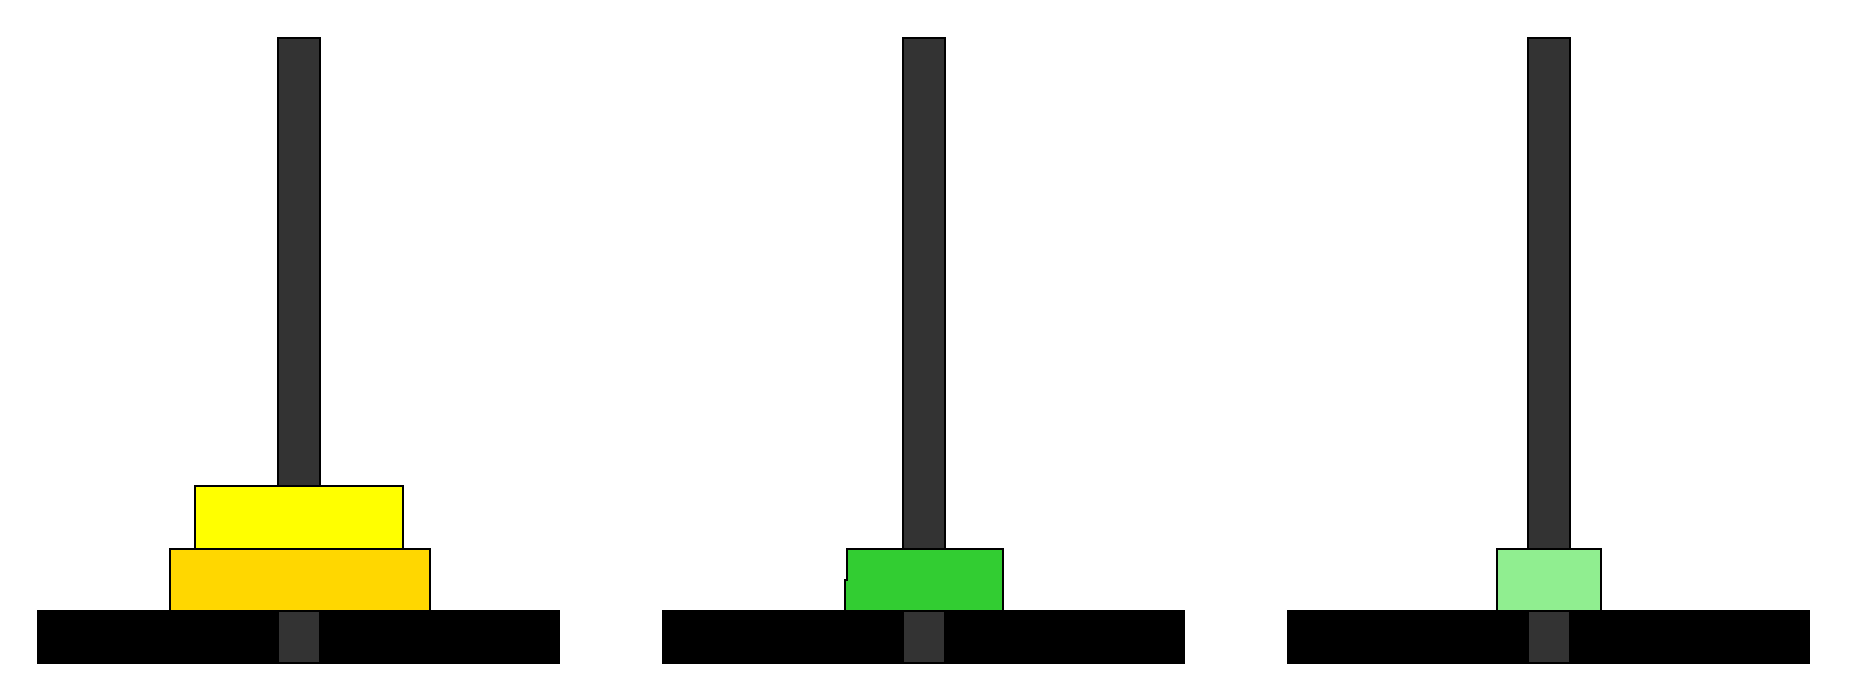
\includegraphics[scale=0.14]{hanoi_dep.eps}
				\end{center}
			\item<3-> Ecrire les opérations permettant de passer la situation précédente à celle ci-dessous :
				\begin{center}
					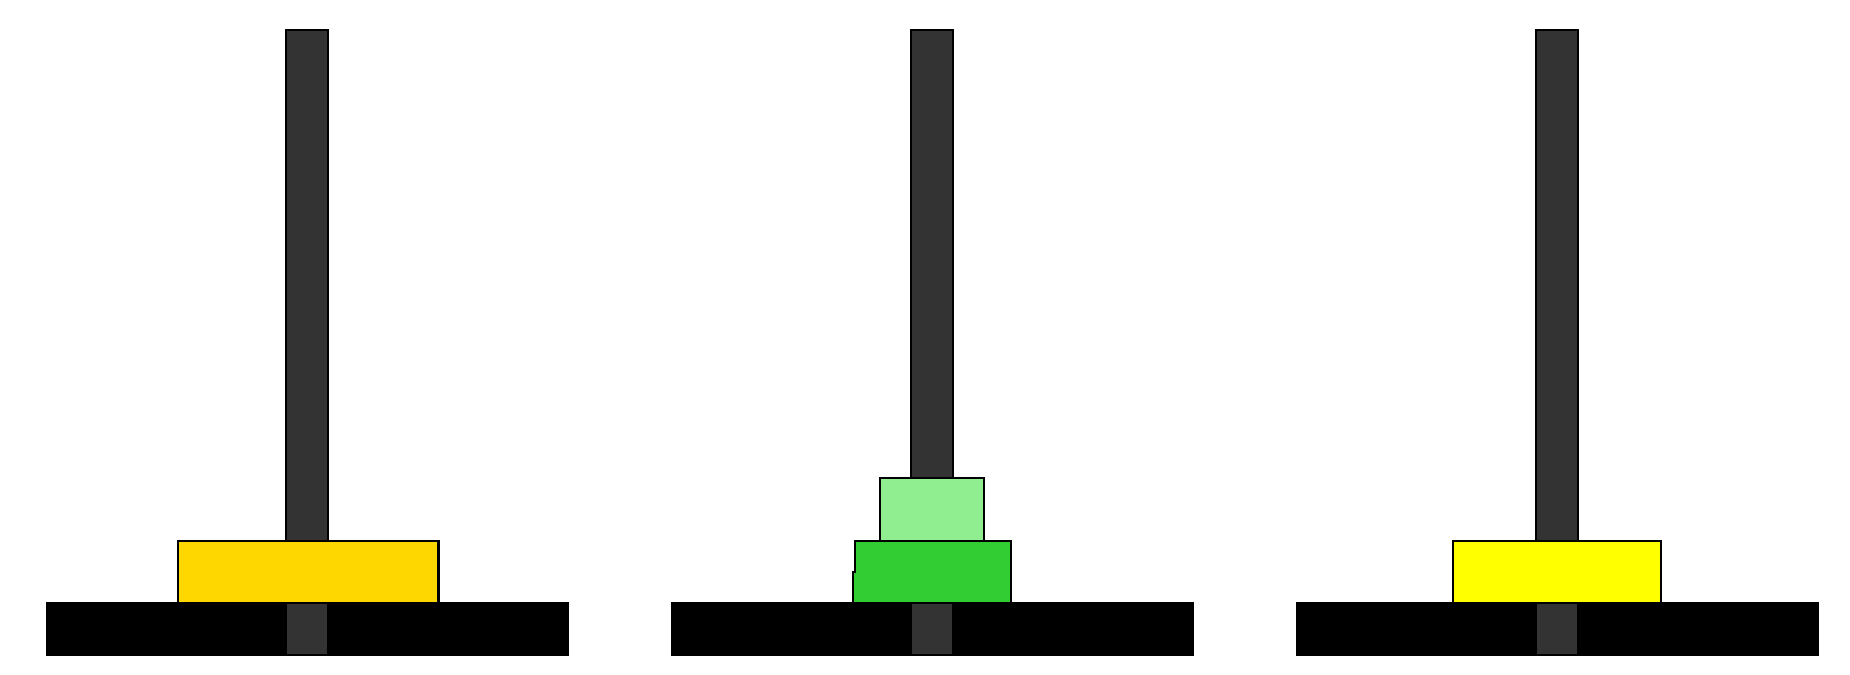
\includegraphics[scale=0.18]{hanoi_fin.eps}
				\end{center}
		\end{enumerate}
	\end{exampleblock}
\end{frame}

\begin{frame}[fragile]{\Ctitle}{\stitle}
	\begin{block}{Implémentation des piles}
		Plusieurs implémentations sont possibles :
		\begin{itemize}
			\item<1-> A l'aide d'une liste chainée, le début de la liste représente alors le sommet. 
			\item<2-> Si la capacité de la pile est bornée et connue en amont, on peut aussi utiliser un tableau et mémoriser la taille {\tt t} de la pile. Puis,
			\begin{itemize}
				\item<3-> pour tester si la pile est vide on teste si {\tt t} est égal à 0,
				\item<4-> pour empiler une valeur {\tt v}, on affecte {\tt tab[t]=v} et on incrémente {\tt t},
				\item<5-> pour dépiler renvoie {\tt tab[t]} et décrémente {\tt t}.
			\end{itemize}
		\end{itemize}
	\end{block}
\end{frame}

% Files : approche sémantique
\makess{Files}
\begin{frame}{\Ctitle}{\stitle}
	\begin{alertblock}{Files}
		\begin{itemize}
			\item<1-> Au niveau sémantique, une \textcolor{blue}{file} est semblable à une file d'attente dans la vie de tous les jours.
				\onslide<2->{\begin{center}
					\onslide<4->{\rnode{enf}{\framebox[1cm]{\tt elt}}}  \hspace{1cm}
					\begin{tabular}{|p{1cm}|p{1cm}|p{1cm}|p{1cm}|}
						\hline
						\rnode{in}{\tt elt4} & {\tt elt3} & {\tt elt2} & \rnode{out}{\tt elt1} \\
						\hline
					\end{tabular}
					\hspace{1cm} \onslide<9->{\rnode{def}{\framebox[1cm]{\tt elt}}}
					}
					\onslide<5->{\ncline[linestyle=dashed,nodesepB=0.2cm]{->}{enf}{in}}
					\onslide<6->{\naput{{\footnotesize \textcolor{blue}{enfiler}}}}
					\onslide<9->{\ncline[linestyle=dashed,nodesepA=0.4cm]{->}{out}{def}}
					\onslide<10->{\naput{{\footnotesize \textcolor{blue}{défiler}}}}
				\end{center}
			\item<3-> Enfiler signifie ajouter un élément en fin de file
			\item<7-> Défiler signifie retirer l'élément situé au début de la file.
			\item<11-> Ainsi le premier élément entré dans la file sera aussi le premier à en sortir, on dit qu'une file est une structure \textcolor{blue}{\sc fifo} \textit{First In First Out}
		\end{itemize}
	\end{alertblock}
\end{frame}



% Files
\begin{frame}{\Ctitle}{\stitle}
	\begin{alertblock}{Files comme structures de données}
		L'interface d'une structure de données File se limite donc aux opérations suivantes :
		\begin{itemize}
			\item<2-> \textcolor{blue}{\tt est\_vide()} qui renvoie un booléen indiquant si la file est vide ou non.
			\item<3-> \textcolor{blue}{\tt enfiler(element)} qui ajoute un élément à la fin de la file.
			\item<4-> \textcolor{blue}{\tt defiler()} qui retire l'élément situé au début de la file (cela n'est possible que si la file n'est pas vide).
		\end{itemize}
	\end{alertblock}
	\onslide<5->{
		\begin{block}{Utilisation}
			Comme pour les piles, cette structure de données a de nombreuses applications en informatique : file d'attente d'une imprimante, simulation de files d'attentes réelles, \dots
		\end{block}}
\end{frame}

% Piles : EX1
\begin{frame}{\Ctitle}{\stitle}
	\begin{exampleblock}{Manipulation de files}
		\begin{itemize}
			\item<2-> On considère la file : {\tt F = >"E","L","S","A">}. Quelle suite d'opération permet d'obtenir {\tt F= >"N","O","E","L">} ?
			\item<3-> On simule la file d'attente d'une imprimante à l'aide d'une file. A quelle opération sur cette file correspond l'envoie d'une nouvelle impression ? La fin de l'impression en cours ? Dans quel ordre seront effectuées les impressions ?
		\end{itemize}
	\end{exampleblock}
\end{frame}


\begin{frame}[fragile]{\Ctitle}{\stitle}
	\begin{block}{Implémentation des files}
		Plusieurs implémentations sont possibles :
		\begin{itemize}
			\item<1-> A l'aide d'une liste chainée, dans ce cas si on veut pouvoir enfiler et défiler en temps constant, il faut disposer d'un accès au premier maillon et au dernier maillon. 
			\item<2-> Si la capacité de la file est bornée et connue en amont, on peut aussi utiliser un tableau de façon circulaire en mémorisant l'indice du début de la file et l'indice de fin.
			\item<3-> On peut aussi implémenter une file avec deux piles. 
		\end{itemize}
	\end{block}
\end{frame}

\end{document}